\documentclass{article}
\usepackage{graphicx}
\usepackage{amsmath}

\usepackage{listings}
\usepackage{color}

\definecolor{backcolour}{rgb}{0.95,0.95,0.92}

\lstdefinestyle{mystyle}{
    backgroundcolor=\color{backcolour}
    }

\lstset{style=mystyle}

\title{Statistical Modeling 2 \\ Exercise 3}

\begin{document}
\maketitle
\section*{Basic concepts}
\begin{align*}
\mbox{MSE}(\hat{f}, f) &= E\{[f(x) - \hat{f}(x)]^2\}\\
&= E [ f(x)^2 + \hat{f}(x)^2 - 2f(x)\hat{f}(x)]\\
&=  f(x)^2 + E[\hat{f}(x)^2] - E[\hat{f}(x)]^2 + E[\hat{f}(x)]^2 - 2 f(x) E[\hat{f}(x)]\\
&= \{E[\hat{f}(x)^2] - E[\hat{f}(x)]^2\} + \{f(x)^2 + E[\hat{f}(x)]^2 - 2 f(x) E[\hat{f}(x)]\}\\
&= V + B^2
\end{align*}


\section*{Curve fitting by linear smoothing}
\subsection*{A}
In the least square estimate, we minimize:
\begin{align*}
L = \sum_{i=1}^n (\hat{\beta}x_i - y_i)^2
\end{align*}
We take the derivative and set to \(0\):
\begin{align*}
\partial L / \partial \hat{\beta} &= \sum_{i=1}^n 2 (\hat{\beta}x_i - y_i) x_i = 0\\
&\implies \hat{\beta}(\sum_{i=1}^n x_i^2) - \sum_{i=1}^n y_i x_i = 0\\
&\implies \hat{\beta} = \frac{\sum_{i=1}^n y_i x_i}{ \sum_{i=1}^n x_i^2}
\end{align*}
We have that the prediction is:
\begin{align*}
\hat{f}(x^*) &= \hat{\beta} x^*\\
&= \frac{\sum_{i=1}^n x_i x^* y_i}{ \sum_{i=1}^n x_i^2}\\
&= \sum_{i=1}^n w(x_i, x^*) y_i 
\end{align*}
where
\begin{align*}
w(x_i, x^*) = \frac{x_i x^*}{ \sum_{i=1}^n x_i^2}
\end{align*}

This weight function weights examples by the product with predictors, using all the points in the dataset. The K nearest function weights the \(K\) nearest neighbors equally and ignore all other points. 

\subsection*{B}
Code: kernel.r


\begin{figure}[h!]
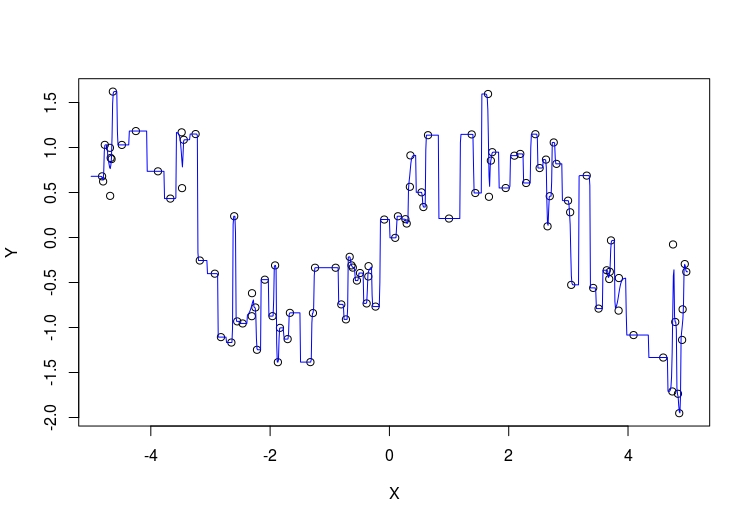
\includegraphics[width = \textwidth]{h001.jpeg}
\caption{Bandwidth \(h = 0.01\)}
\end{figure}

\begin{figure}[h!]
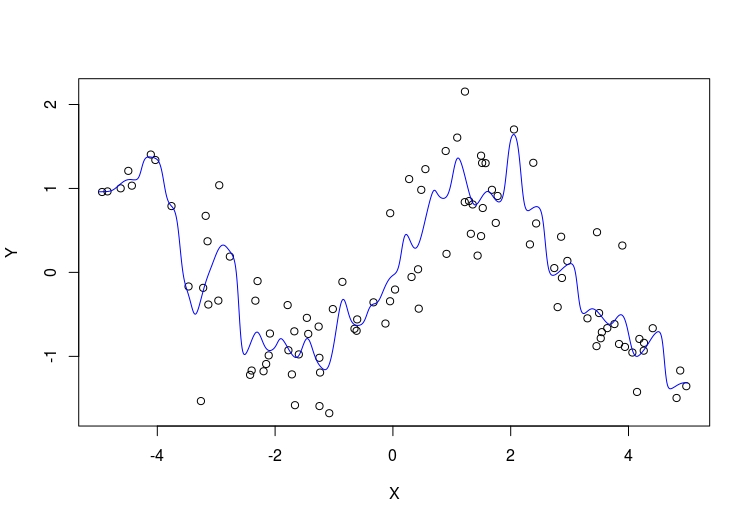
\includegraphics[width = \textwidth]{h01.jpeg}
\caption{Bandwidth \(h = 0.1\)}
\end{figure}


\begin{figure}[h!]
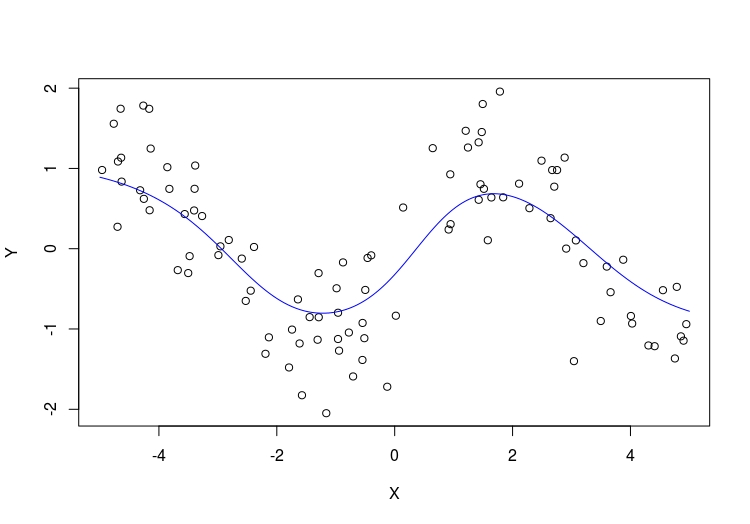
\includegraphics[width = \textwidth]{h1.jpeg}
\caption{Bandwidth \(h = 1\)}
\end{figure}

The bandwidth \(h\) affects the smoothness of the prediction line. With smaller \(h\), more weight is given to neighbor points and the line fluctuates. With larger \(h\), more weight is given to points that are further away, resulting in a smoother line.

\section*{Cross Validation}
\subsection*{B}

\begin{figure}[h!]
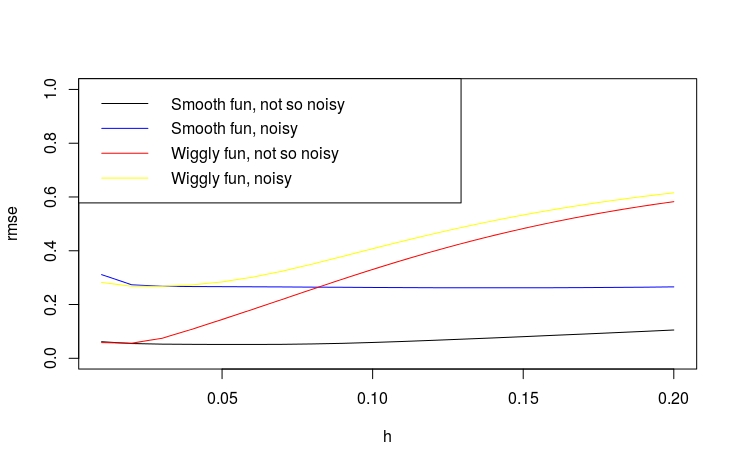
\includegraphics[width = \textwidth]{cv.jpeg}
\caption{Cross Validation}
\end{figure}


\end{document}